\begin{boldmath}
\chapter{Limits on $q^*$ production at a VLHC}
\label{chap:VLHC_Qstar}
\end{boldmath}

\input QstarVLHC/authorlist.tex

We look for a dijet resonance corresponding to an excited quark $q^*$
in a simulated sample corresponding to 3\,ab$^{-1}$ of $pp$ collisions
at $\sqrt{s} = 100$\,TeV.  Using a cut and count analysis approach we
are able to exclude $q^*$ masses upto 48\,TeV at 95\% CL,
corresponding to a length scale of around 4\,am.

\section{Introduction}

At the new energy regime afforded by a $\sqrt{s} =100$\,TeV $pp$
collider (VLHC), we search for possible structure to the quarks of the
standard model \cite{Baur:1989kv, Baur:1987ga, Harris:1996ct}.  The primary background for a
signal of this type is the QCD dijet production.

\section{Data and detector simulation}

We utilize \textsc{pythia} and the CTEQ6L1 PDF's to genererate both
background and signal events and provide parton showering.  The center
of mass energy of the $pp$ collisions is 100\,TeV.  We use the
``Snowmass'' detector~\cite{SnowDet}, based on the
Delphes~\cite{Delphes} detector simulation package, to simulate the
detector response.  The foreseen rate for ``pile-up'' $pp$
interactions is an average of 140 minimum bias interactions per bunch
crossing.  The integrated liminosity is expected to reach
3\,ab$^{-1}$.  During the production of the signal samples, we use the
convention $\Lambda = m_{q^*}$.  The cross-sections reported by
\textsc{pythia} for the considered processes are contained in
Table~\ref{tab:qstar_xsec}.

\begin{table}
\caption{\label{tab:qstar_xsec} Cross-sections for signal processes.}
\begin{center}
\begin{tabular}{|c|c|}
\hline
$q^*$ mass & cross-sections (fb) \\
\hline
30\,TeV & 22.8 \\
40\,TeV & 0.986 \\
50\,TeV & $4.38\times 10^{-2}$ \\
60\,TeV & $2.22\times 10^{-3}$ \\
\hline
\end{tabular}
\end{center}
\end{table}

\section{Analysis}

Within the sample, we select the two jets with the largest
$p_\mathrm{T}$.  To reduce the relative contribution of the QCD dijet
production, we require that the jet $p_\mathrm{T} > 10$\,TeV and $|\eta
| < 1.0$.  We use the dijet invariant mass spectrum to separate the
signal and background components.  The mass spectrum for the
background and various signals is shown in
Fig.~\ref{fig:qstar_vlhc}(left).  

Because of the huge cross-section for the QCD process, we parameterize
the spectral shape from a large sample of simulated events and scale
this shape to provide our background estimate.  The functional form
selected for the background is a exponential decay with an error
funtion turn-on at the low mass end of the specturm.  The line-shapes
for the various signal hypotheses are parameterized by a Gaussian
shape for the peak and a wide structure to capture poorly
reconstructed events.

Limits are derived using a simple counting method.  We select a signal
window corresponding to $\pm 2\sigma$ of the peaking component of the
signal.  Using the signal and background counts within the signal
window, we place an asymptotic 95\% CL upper limit on the
cross-section for a given $q^*$ mass.  In these limits we do not
include any systematic uncertainties.  Given the simplicity of this
analysis, degradations due to systematic uncertainties can be
compensated through more advanced analysis techniques.

\section{Results}

\begin{figure}
\begin{center}
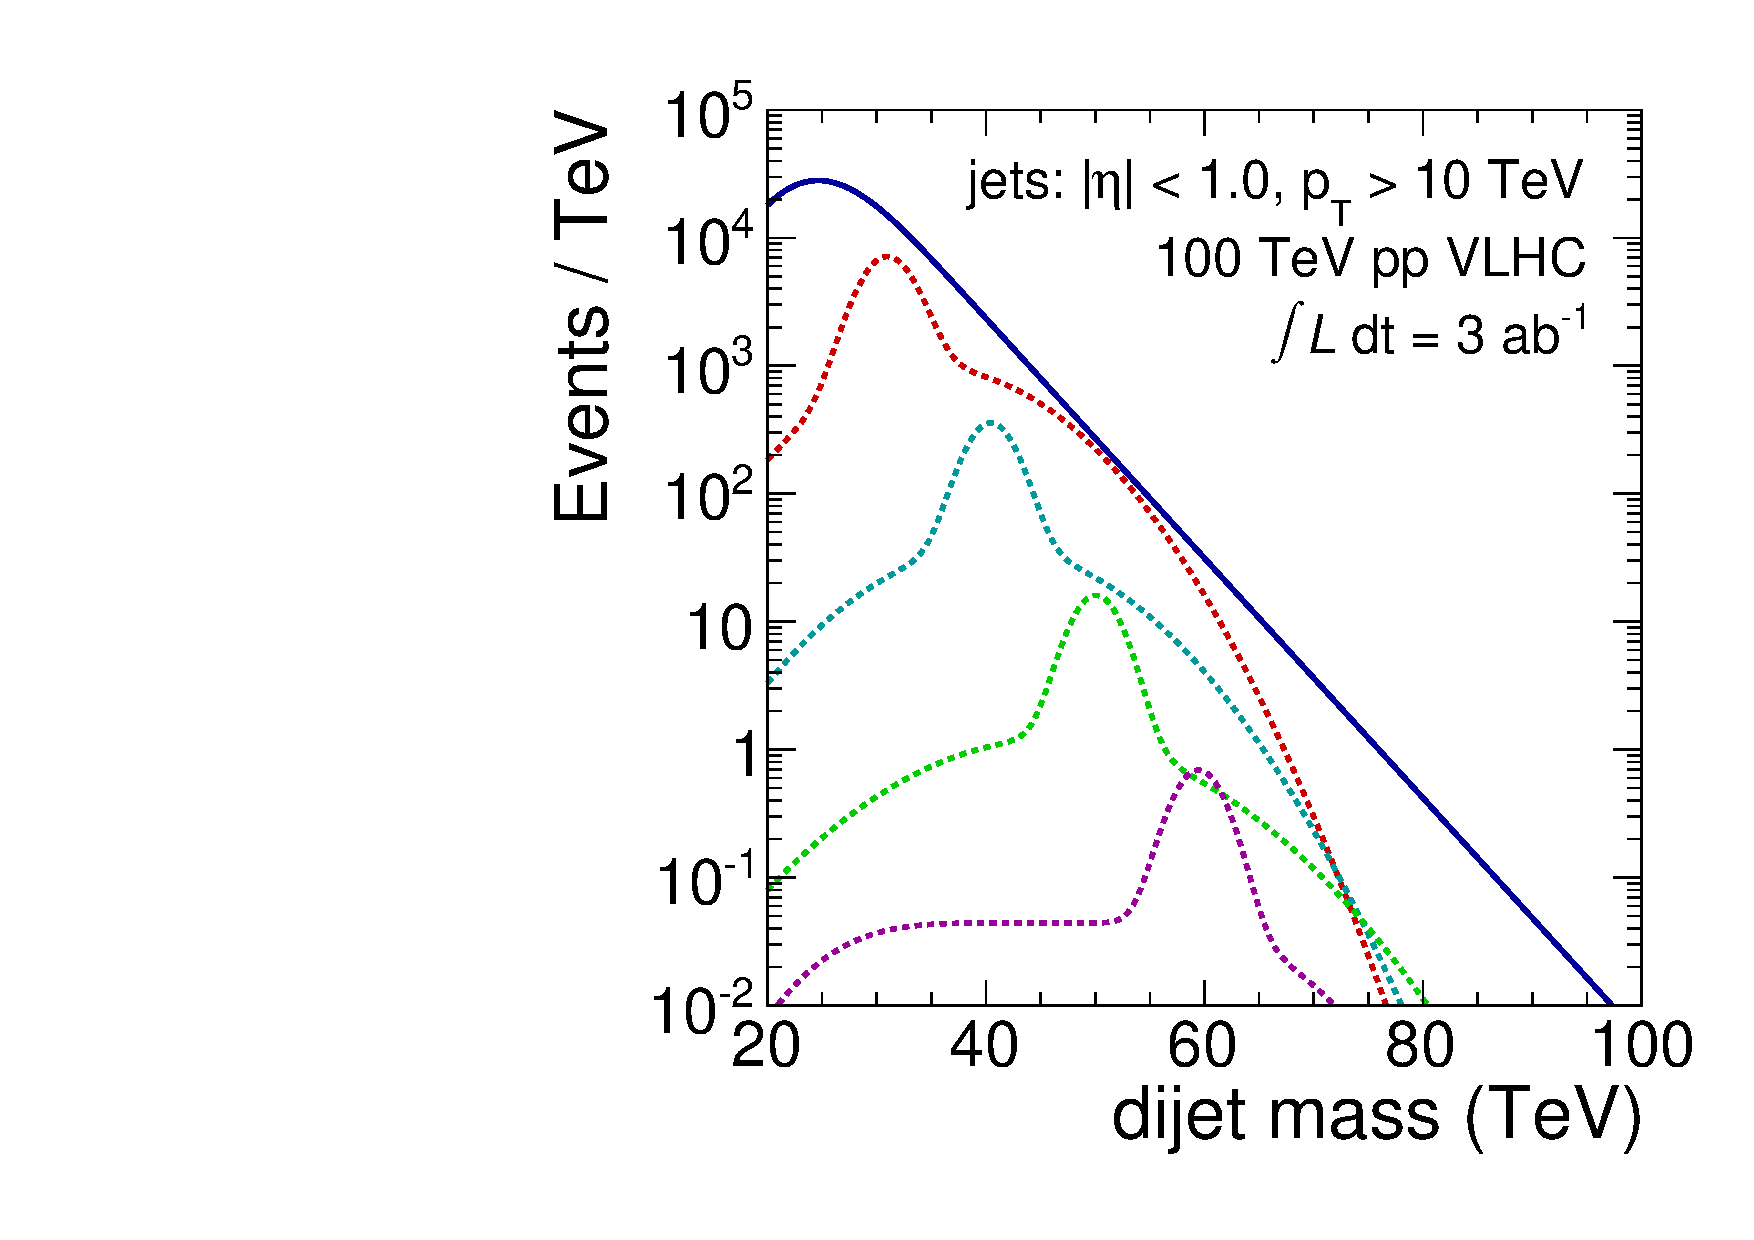
\includegraphics[width=0.475\textwidth]{QstarVLHC/plots/qstar_100TeV}
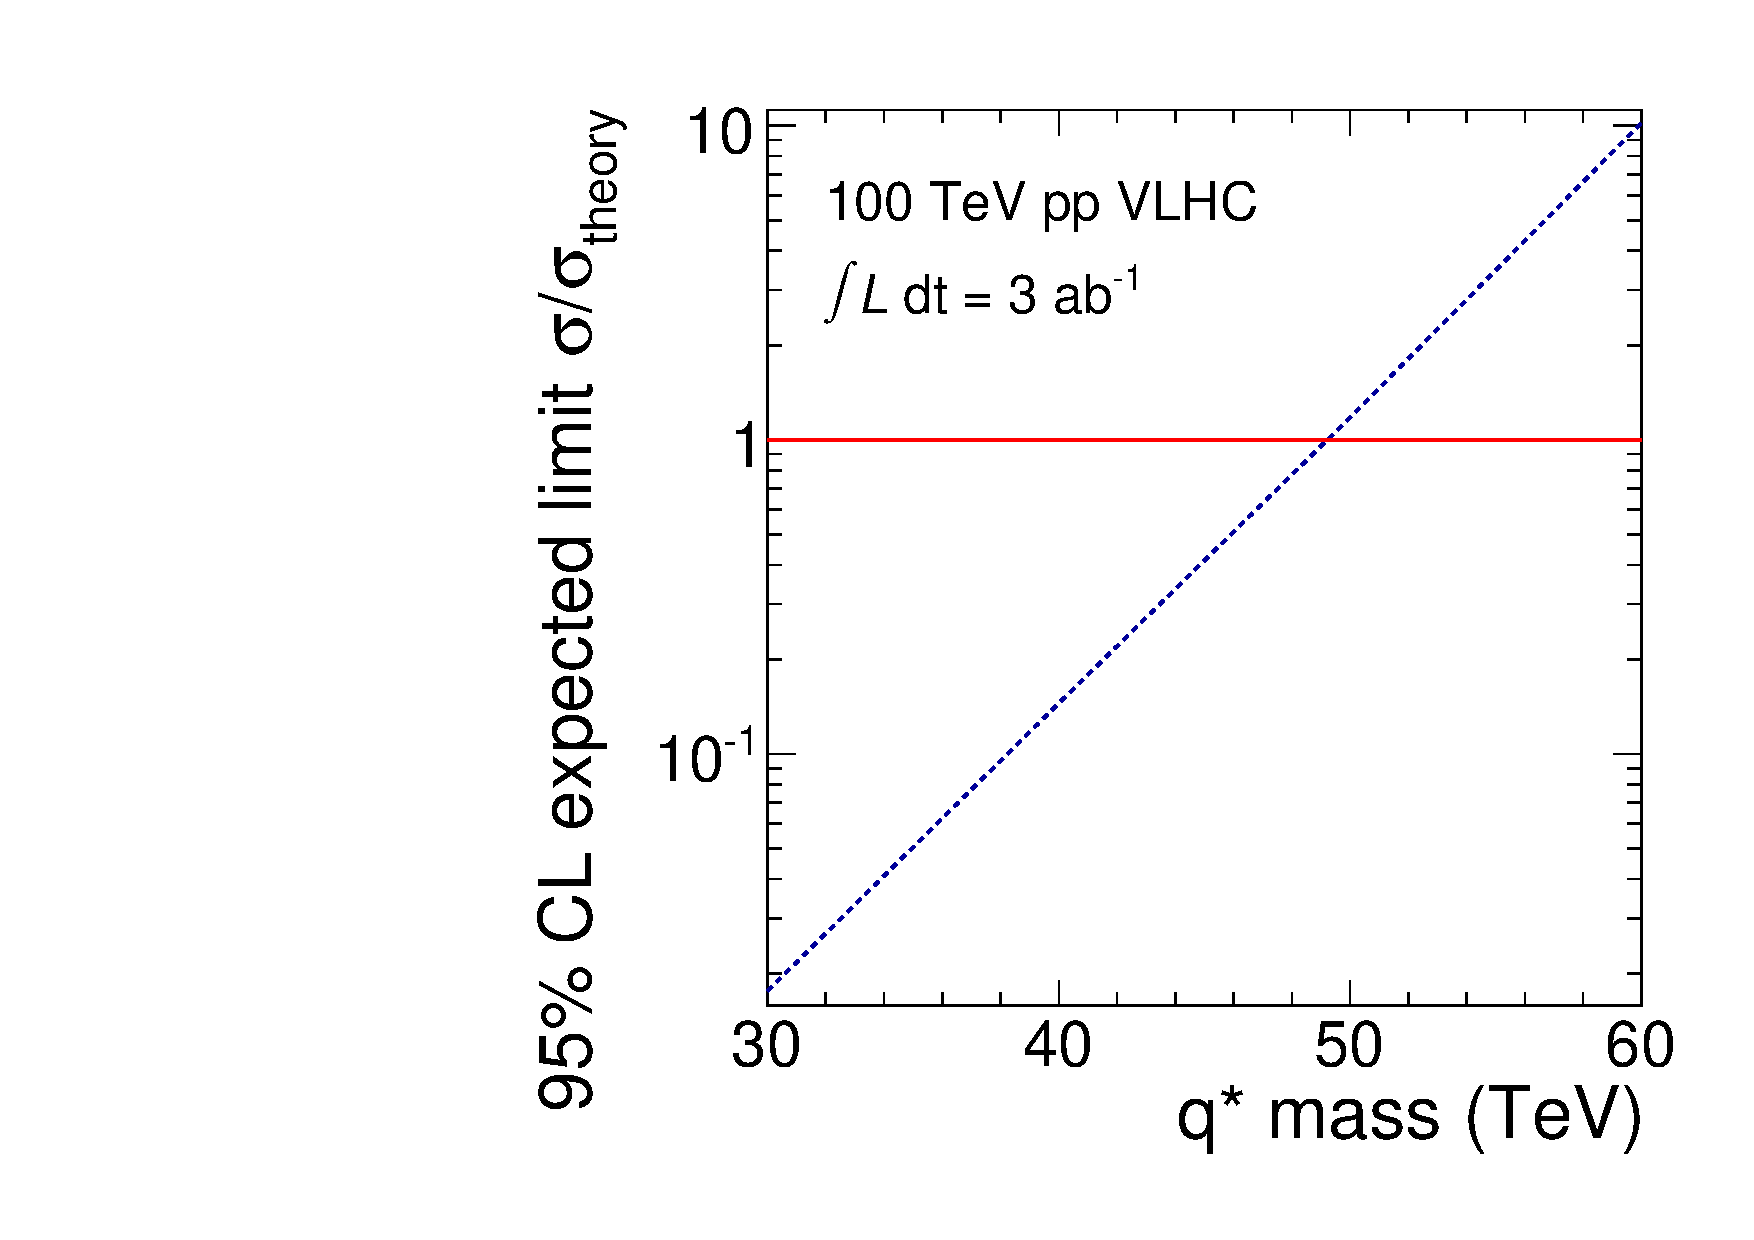
\includegraphics[width=0.475\textwidth]{QstarVLHC/plots/qstar_limits}
\end{center}
\caption{\label{fig:qstar_vlhc}(left) Dijet mass spectrum for
  background dijet production (solid blue line) and $q^*$ models with
  masses from 30\,TeV to 60\,TeV (dashed colored lines). (right) 95\%
  CL upperlimit on the cross-section of $q^*$ resonance as a function
  of its mass normalized by the theoretical prediction for the
  cross-section.}
\end{figure}

Figure~\ref{fig:qstar_vlhc}(right) shows the expected limit as a
function of $q^2$ mass.  We can expect to exclude masses upto 48\,TeV
using the full luminosity of the a VLHC.  A reach of 48\,TeV would
exclude structure of quarks on the order of 4\,am.

\begin{thebibliography}{99}

\bibitem{Baur:1989kv} 
  U.~Baur, M.~Spira and P.~M.~Zerwas,
  %``Excited Quark And Lepton Production At Hadron Colliders,''
  Phys.\ Rev.\ D {\bf 42}, 815 (1990).

\bibitem{Baur:1987ga} 
  U.~Baur, I.~Hinchliffe and D.~Zeppenfeld,
  %``Excited Quark Production at Hadron Colliders,''
  Int.\ J.\ Mod.\ Phys.\ A {\bf 2}, 1285 (1987).
  %%CITATION = IMPAE,A2,1285;%%
  %118 citations counted in INSPIRE as of 29 Aug 2013

\bibitem{Harris:1996ct} 
  R.~M.~Harris,
  %``Discovery mass reach for excited quarks at hadron colliders,''
  eConf C {\bf 960625}, NEW164 (1996)
  [hep-ph/9609319].
  %%CITATION = HEP-PH/9609319;%%
  %7 citations counted in INSPIRE as of 29 Aug 2013

\bibitem{Delphes} 
  J.~de Favereau, C.~Delaere, P.~Demin, A.~Giammanco, V.~Lemaître, A.~Mertens and M.~Selvaggi,
  %``DELPHES 3, A modular framework for fast simulation of a generic collider experiment,''
  arXiv:1307.6346 [hep-ex].
  %%CITATION = ARXIV:1307.6346;%%
  %9 citations counted in INSPIRE as of 29 Aug 2013

\end{thebibliography}


